%%%%%%%%%%%%%%%%%%%%%%%%%%%%%%%%%%%%%%%%%%%%%%%%%%%%%%%%
\fondo{celeste}
\section{Convolución}
\fondo{blanco}
%%%%%%%%%%%%%%%%%%%%%%%%%%%%%%%%%%%%%%%%%%%%%%%%%%%%%%%%

%%%%%%%%%%%%%%%%%%%%%%%%%%%%%%%%%%%%%%%%%%%%%%%%%%%%%%%%
\begin{frame}
    \begin{block}{Convolución}
        La convolución entre dos funciones \( f \) y \( g \) se define como:
        \[
        s(t) = (f \ast g)(t) = \int_{-\infty}^{+\infty} f(\tau) g(t - \tau) \, d\tau
        \]
    \end{block}
    
    \begin{itemize}
        \item \( f \) es la función de entrada.
        \item \( g \) es el filtro o kernel.
    \end{itemize}
\end{frame}
%%%%%%%%%%%%%%%%%%%%%%%%%%%%%%%%%%%%%%%%%%%%%%%%%%%%%%%%


%%%%%%%%%%%%%%%%%%%%%%%%%%%%%%%%%%%%%%%%%%%%%%%%%%%%%%%%
\begin{frame}
    \begin{block}{Convolución Discreta}
        Para datos discretos, la convolución se define como:
        \[
        s(t) = (f \ast g)(t) = \sum_{\tau = -\infty}^{\infty} f(\tau) g(t - \tau)
        \]
    \end{block}
    
    \begin{block}{Convolución en Dos Dimensiones (Imágenes)}
        La convolución entre una imagen \( I \) y un kernel \( K \) es:
        \[
        S(i, j) = (I \ast K)(i, j) = \sum_m \sum_n I(i - m, j - n) K(m, n)
        \]
    \end{block}
\end{frame}
%%%%%%%%%%%%%%%%%%%%%%%%%%%%%%%%%%%%%%%%%%%%%%%%%%%%%%%%


%%%%%%%%%%%%%%%%%%%%%%%%%%%%%%%%%%%%%%%%%%%%%%%%%%%%%%%%
\begin{frame}
    \begin{block}{Correlación Cruzada}
        La correlación cruzada entre una imagen \( I \) y un kernel \( K \) es:
        \[
        S(i, j) = (I \ast K)(i, j) = \sum_m \sum_n I(i + m, j + n) K(m, n)
        \]
    \end{block}

    \begin{itemize}
        \item 
        En la práctica, se usa correlación cruzada en lugar de convolución.
        \item 
        La correlación cruzada evita invertir el kernel, lo que simplifica la implementación
    \end{itemize}
\end{frame}
%%%%%%%%%%%%%%%%%%%%%%%%%%%%%%%%%%%%%%%%%%%%%%%%%%%%%%%%



%%%%%%%%%%%%%%%%%%%%%%%%%%%%%%%%%%%%%%%%%%%%%%%%%%%%%%%%
\begin{frame}[fragile]
    \footnotesize
    \begin{tikzpicture}
        % Input matrix
        \matrix[matrix of math nodes, nodes={draw, minimum size=0.7cm, anchor=center, fill=celeste!20},column sep=-\pgflinewidth,row sep=-\pgflinewidth] (m1) {
            a & b & c & d \\
            e & f & g & h \\
            i & j & k & l \\
        };
    
        % Kernel matrix
        \matrix[matrix of math nodes, nodes={draw, minimum size=0.7cm, anchor=center, fill=gray!40},column sep=-\pgflinewidth,row sep=-\pgflinewidth] (m2) [right=0.5cm of m1] {
            w & x \\
            y & z \\
        };
    
        % Output matrix
        \matrix[matrix of math nodes,nodes={draw, minimum size=0.7cm, minimum width=3cm, anchor=center},column sep=-\pgflinewidth,row sep=-\pgflinewidth] (m3) [right=0.5cm of m2] {
            aw+bx+ey+fz & bw+cx+fy+gz & cw+dx+gy+hz \\
            ew+fx+iy+jz & fw+gx+jw+kz & gw+hx+ky+lz \\
        };
    
        % Labels
        \node[below=0.2cm of m1] {Input ($3\times4$)};
        \node[below=0.2cm of m2] {Kernel ($2\times2$)};
        \node[below=0.2cm of m3] {Output ($2\times3$)};
    
        % Dashed boxes around convolution areas
        \draw[red, thick, dashed] ($(m1-1-1.north west)+(-0.1,0.1)$)  rectangle ($(m1-2-2.south east)+(0.1,-0.1)$);
        \draw[red, thick, dashed] ($(m2-1-1.north west)+(-0.1,0.1)$)  rectangle ($(m2-2-2.south east)+(0.1,-0.1)$);
        \draw[red, thick, dashed] ($(m3-1-1.north west)+(-0.1,0.1)$) rectangle ($(m3-1-1.south east)+(0.1,-0.1)$);
    
        % Arrows
        \draw[red, thick, ->] ($(m1-1-1.north east)+(0,0.1)$) to[out=10, in=150] ($(m3-1-1.north)+(0.4,0.1)$);
        \draw[red, thick, ->] ($(m2-1-1.north east)+(0,0.1)$) to[out=10, in=140] ($(m3-1-1.north)+(-0.4,0.1)$);
    
        % Operations
        \node[right=-0.05cm of m1] {\large $*$};
        \node[right=-0.05cm of m2] {\large $=$};
        
    \end{tikzpicture}
\end{frame}

\begin{frame}{Filtros}

    \vspace*{-2.5cm}
    \begin{columns}
    \column{3cm}
        
        \href{https://mlnotebook.github.io/img/CNN/convSobel.gif}{Ver animación.}
        
    \column{8cm}
    \begin{center}
        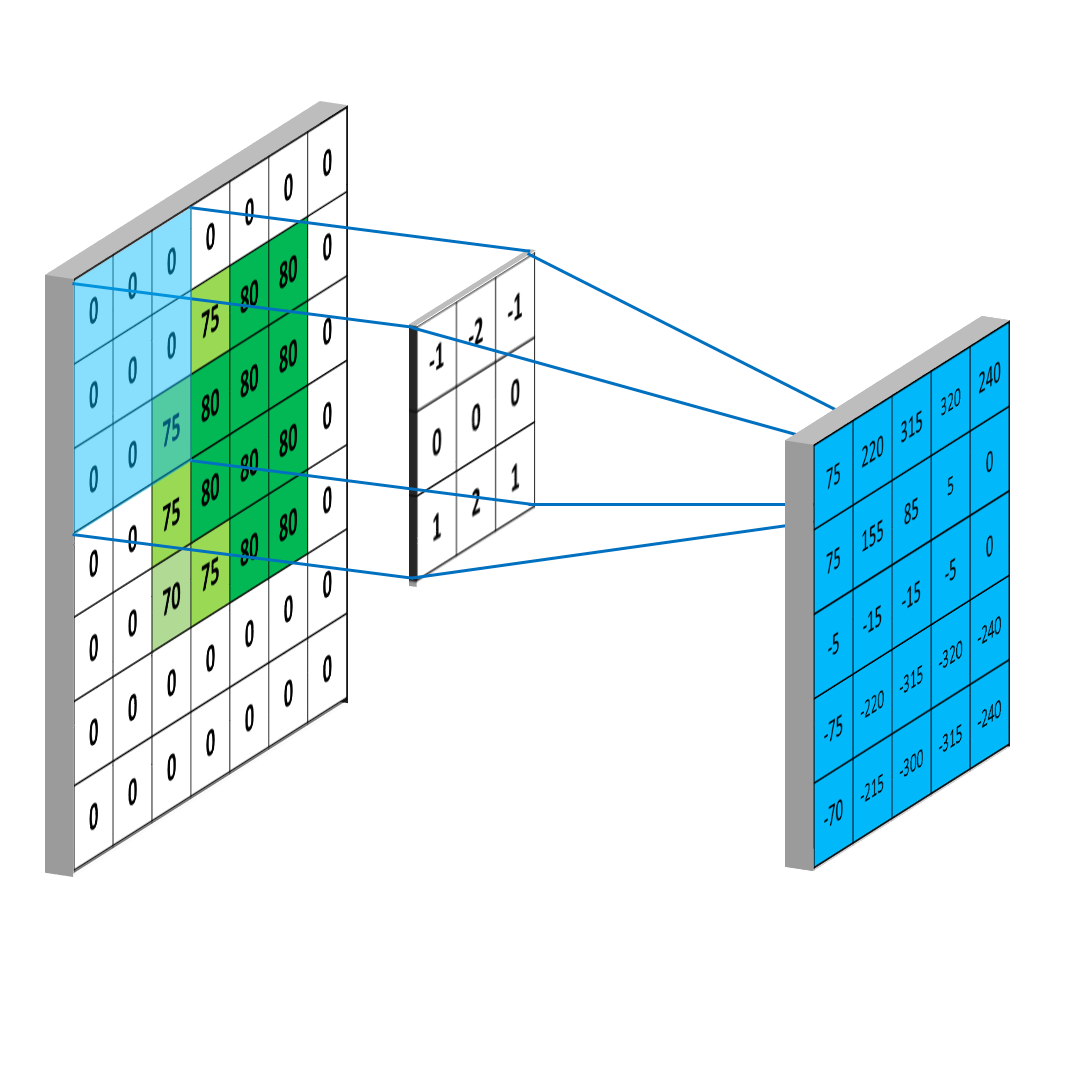
\includegraphics[height=9.5cm]{Figuras/Fig10}
    \end{center}
    \end{columns}
    
\end{frame}

%%%%%%%%%%%%%%%%%%%%%%%%%%%%%%%%%%%%%%%%%%%%%%%%%%%%%%%%
\begin{frame}

    La dimensión de salida después de aplicar una convolución es:
    \[
        (I_1 - K_1 + 1,\ I_2 - K_2 + 1),
    \]
    dónde
    \begin{itemize}
        \item 
        \( I_1, I_2 \) son las dimensiones de la imagen de entrada, y 
        \item 
        \( K_1, K_2 \) son las dimensiones del kernel
    \end{itemize}
\end{frame}
%%%%%%%%%%%%%%%%%%%%%%%%%%%%%%%%%%%%%%%%%%%%%%%%%%%%%%%%
